\chapter{Introduction}

\section{Divers débits}
\begin{figure}[H]
    \centering
    \subfigure[\label{fig:debitEtiage} Etiage \textit{ou basse eau} (\LS{15})]{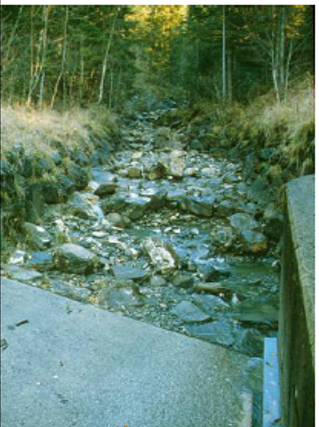
\includegraphics[height=7cm]{etiage.png}}
    \subfigure[\label{fig:debitNormal} Débit normal \textit{ou morphogène} (\MH{0.7})]{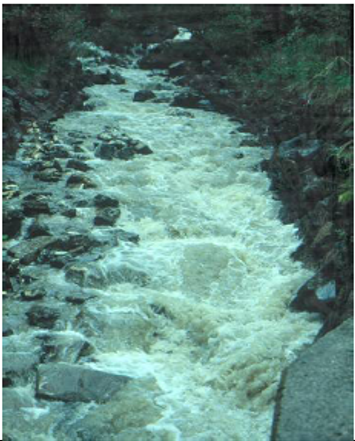
\includegraphics[height=7cm]{debitNormal.png}}
    \subfigure[\label{fig:debitCrue} Crues (\MH{10})]{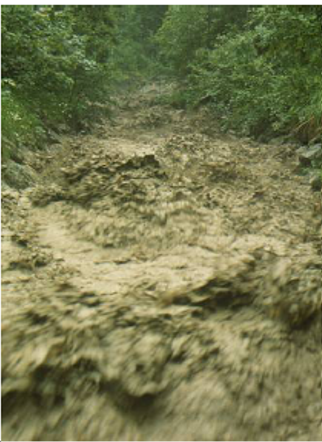
\includegraphics[height=7cm]{crue.png}}
    \caption{Différentes dénominations de débits}
    \label{fig:debits}
\end{figure}

\begin{itemize}
    \item \underline{\textbf{Débit d'étiage :}} quand les rivières tombent à sec ou presque.
    Il est important de connaître ces valeurs minimales dans un cours pour gérer toutes les demandes en matière de prélèvement d'eau, d'écoulement permanent à restituer en aval d'un barrage.
    La législation suisse parle d'un débit $Q_{347}$ (débit moyen sur une journée dépassé en moyenne 347 jours dans une année).
    \item \underline{\textbf{Débit morphogène :}} les érosions des berges sont normalement influencées par ces mêmes débits. Cela dépend aussi des caractéristiques locales comme la granulométrie du fond du lit.
    \item \underline{\textbf{Crue :}} important de connaître le débit pour pouvoir définir les zones de risques au sens de la législation suisse (cf. unité de cours \texttt{Hydraulique 2}).
\end{itemize}

\section{Débits et temps de retour}
\begin{itemize}
    \item Une crue qui survient en moyenne 1 fois tous les 100 ans affiche donc un temps de retour centennal.
    On peut aussi parler de $Q_{100}$.
    \item La probabilité moyenne associée à ce temps de retour d'être atteinte ou dépassée est de 1/100.
    \item Les lois et recommandations fédérales obligent des protections en fonction des temps de retours (cf. Figure \ref{fig:matriceProtection}).
\end{itemize}
\begin{figure}[h!]
    \centering
    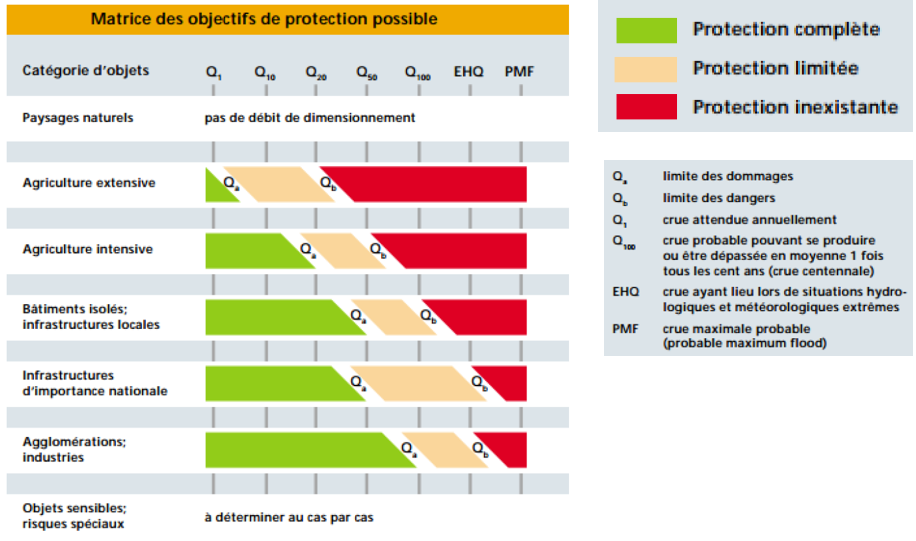
\includegraphics[width=10cm]{matriceObjectifsDimensionnement.png}
    \caption{Matrice de protection possible}
    \label{fig:matriceProtection}
\end{figure}

\section{Méthodes d'analyse et de calculs}
\begin{enumerate}
    \item Analyse statistique avec veille hydrologique
    \item Modèle conceptuel avec des corrélations exprimant les débits de dimensionnement en fonction des paramètres physiques et morphologiques du bassin versant
\end{enumerate}